\begin{figure}[H]
    \centering
    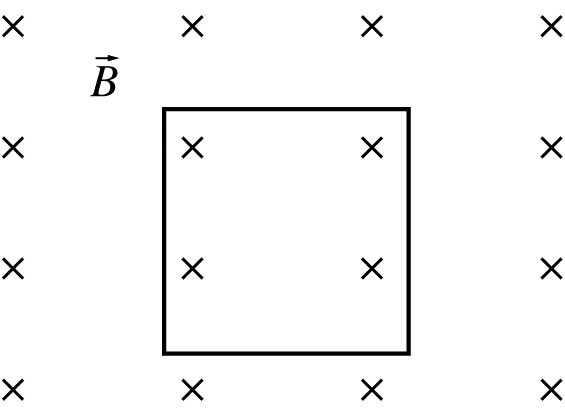
\includegraphics[scale=0.3]{images/img-005-008.png}
\end{figure}

% Multiple Choice Question 8
\begin{questions}\setcounter{question}{7}\question
A loop of wire lies in the plane of the page in a region with a uniform magnetic field $\vec{B}$ directed into the page, as shown in the figure above. In which of the following cases, if any, will an emf be induced in the loop at the moment shown in the figure?

\begin{choices}
\choice The loop is moving toward the right.
\choice The loop is moving toward the top of the page.
\choice The loop is moving out of the plane of the paper so that the loop's plane remains perpendicular to the magnetic field.
\choice The loop is moving into the plane of the paper so that the loop's plane remains perpendicular to the magnetic field.
\choice An emf cannot be induced in the loop without changing its orientation relative to the magnetic field.
\end{choices}\end{questions}
